\section{Model Description}

The gravity effector module is responsible for calculating the effects of gravity from a body on a spacecraft. A spherical harmonics model and implementation is developed and described below. The iterative methods used for the software algorithms are also described. Finally, the results of the code unit tests are presented and discussed.

\subsection{Mathematical model}

\subsubsection{Gravity models}

Gravity models are usually based on solutions of the Laplace equation ($\nabla^2 U(\mathbf{\bar r}) = 0$). It is very important to state that this equation only models a gravity potential outside a body. For computing a potential inside a body the Poisson equation is used instead.

The spherical harmonic potential is a solution of the Laplace equation using orthogonal spherical harmonics. It can be derived solving the Laplace equation in spherical coordinates, using the separation of variables technique and solving a Sturm-Liouville problem. In this work, the solution will be found using another technique, which essentially follows Vallado's book\cite{vallado2013}.

For each element of mass $d m_\text{Q}$ the potential can be written as
\begin{equation}
\D U(\mathbf{\bar r}) = G \frac{\D m_\text{Q}}{\rho_\text{Q}}
\end{equation}

where $\rho_\text{Q}$ is the distance between the element of mass and the position vector $\mathbf{\bar r}$ where the potential is computed. This position vector is usually given in a body-fixed frame. The relation between the position vector $\mathbf{\bar r}$, the position of the element of mass $\mathbf{\bar r_\text{Q}}$ and $\rho_\text{Q}$ can be given using the cosine theorem and the angle $\alpha$ between the two position vectors, as can be appreciated in Figure \ref{fig:spher_harm}.

\begin{figure}
	\centering
	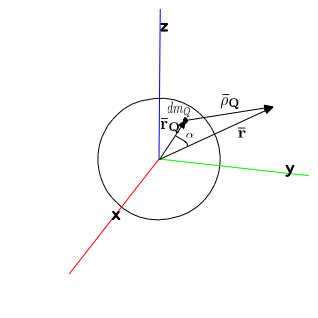
\includegraphics[width=0.3\textwidth]{Figures/spherical_harmonics.png}
	\caption{Geometry of the Spherical Harmonics Representation.}\label{fig:spher_harm}
\end{figure}

\begin{equation}
\rho_\text{Q} = \sqrt{r^2 + r_\text{Q}^2 - 2 r r_\text{Q} \cos(\alpha)} = r \sqrt{1 - 2 \frac{r_\text{Q}}{r} \cos(\alpha) + \bigg(\frac{r_\text{Q}}{r}\bigg)^2} = r \sqrt{1 - 2 \gamma \cos(\alpha) + \gamma^2}
\end{equation}
where $\gamma = r_\text{Q}/r$.

The potential can be obtained by integrating $dU$ through the whole body.
\begin{equation}
U(\mathbf{\bar r}) = G \int_{body} \frac{\D m_\text{Q}}{r \sqrt{1 - 2 \gamma \cos(\alpha) + \gamma^2}}
\end{equation}

If the potential is computed outside the body, $\gamma$ will always be less than 1, and the inverse of the square root can be approximated using the Legendre polynomials $P_l[\beta]$\cite{vallado2013}. Even though this derivation does not use the Laplace equation, it still assumes that the potential is computed outside the body.

The Legendre polynomials can be written as
\begin{equation}
P_l[\beta] = \frac{1}{2^l l!} \frac{d^l}{d \beta^l} (\beta^2 - 1)^l
\end{equation}

The potential is
\begin{equation}
U(\mathbf{\bar r}) = \frac{G}{r} \int_{body} \sum_{l=0}^\infty \gamma^l P_l[\cos(\alpha)] \D m_\text{Q}
\end{equation}

The angle $\alpha$ must be integrated. However, the cosine of the angle $\alpha$ can be decomposed using the geocentric latitude and the longitude associated to vectors $\mathbf{\bar r}$ and $\mathbf{\bar r_\text{Q}}$. These angles will be called $(\phi, \lambda)$ and $(\phi_\text{Q}, \lambda_\text{Q})$ respectively. Using the addition theorem it is possible to write\cite{vallado2013}.
\begin{equation}
P_l[cos(\alpha)] = P_l[\sin(\phi_\text{Q})] P_l[\sin(\phi)] + 2 \sum_{m=1}^l \frac{(l-m)!}{(l+m)!} (a_{l,m} a'_{l,m} + b_{l,m} b'_{l,m})
\end{equation}

where
\begin{align}
	a_{l,m} &= P_{l,m}[\sin(\phi_\text{Q})] \cos(m \lambda_\text{Q})\\
	b_{l,m} &= P_{l,m}[\sin(\phi_\text{Q})] \sin(m \lambda_\text{Q})\\
	a'_{l,m} &= P_{l,m}[\sin(\phi)] \cos(m \lambda)\\
	b'_{l,m} &= P_{l,m}[\sin(\phi)] \sin(m \lambda)
\end{align}

where $P_{l,m}[x]$ are the associated Legendre functions. "$l$" is called degree and "$m$", order. The polynomials can be computed as
\begin{equation}
P_{l,m}[\beta] = (1 - \beta^2)^\frac{m}{2} \frac{d^m}{d \beta^m} P_l[\beta]\label{eq:legendre}
\end{equation}

As can be seen, $a_{l,m}$ and $b_{l,m}$ must be integrated, but $a'_{l,m}$ and $a'_{l,m}$ can be taken outside the integral.
Therefore, it is possible to define
\begin{align}
	C'_{l,m} &= \int_{body} (2 -\delta_m) r_\text{Q}^l \frac{(l-m)!}{(l+m)!} a_{l,m} \D m_\text{Q}\\
	S'_{l,m} &= \int_{body} (2 -\delta_m) r_\text{Q}^l \frac{(l-m)!}{(l+m)!} b_{l,m} \D m_\text{Q}
\end{align}
where $\delta_m$ is the Kronecker delta.

Then
\begin{equation}
U(\mathbf{\bar r}) = \frac{G}{r} \sum_{l=0}^\infty C'_{l,0} \frac{P_l[\sin(\phi)]}{r^l} + \frac{G}{r} \sum_{l=0}^\infty \sum_{m=1}^l \frac{P_{l,m}[\sin(\phi)]}{r^l} \big[C'_{l,m} \cos(m \lambda) + S'_{l,m} \sin(m \lambda)]
\end{equation}

Non-dimensional coefficients $C_{l,m}$ and $S_{l,m}$ are usually used
\begin{align}
	C'_{l,m} &= C_{l,m} R_{\text{ref}}^l m_\text{Q}\\
	S'_{l,m} &= _\text{CoM}S_{l,m} R_{\text{ref}}^l m_\text{Q}
\end{align}
where $m_\text{Q}$ is the total mass of the body and $R_{\text{ref}}$ is a reference radius. If the coefficients $C_{l,m}$ and $S_{l,m}$ are given, the reference radius must be specified. Usually, the reference is chosen as the maximum radius or the mean radius\cite{scheeres2012}.

The potential is then
\begin{equation}
U(\mathbf{\bar r}) = \frac{\mu}{r} \sum_{l=0}^\infty C_{l,0} \bigg(\frac{R_{\text{ref}}}{r}\bigg)^l P_l[\sin(\phi)] + \frac{\mu}{r} \sum_{l=0}^\infty \sum_{m=1}^l \bigg(\frac{R_{\text{ref}}}{r}\bigg)^l P_{l,m}[\sin(\phi)] \big[C_{l,m} \cos(m \lambda) + S_{l,m} \sin(m \lambda)\big]
\end{equation}

Since $P_l[x] = P_{l,0}[x]$ the potential can be written in a more compact way
\begin{equation}
U(\mathbf{\bar r}) = \frac{\mu}{r} \sum_{l=0}^\infty \sum_{m=0}^l \bigg(\frac{R_{\text{ref}}}{r}\bigg)^l P_{l,m}[\sin(\phi)] \big[C_{l,m} \cos(m \lambda) + S_{l,m} \sin(m \lambda)\big]
\end{equation}

Some coefficients have a very interesting interpretation. 
\begin{align}
	C_{0,0} &= 1\\
	S_{l,0} &= 0 \quad \forall l \geq 0\\
	C_{1,0} &= \frac{Z_{\text{CoM}}}{R_{\text{ref}}}\\
	C_{1,1} &= \frac{X_{\text{CoM}}}{R_{\text{ref}}}\\
	S_{1,1} &= \frac{Y_{\text{CoM}}}{R_{\text{ref}}}
\end{align}

where $[X_\text{CoM}, Y_\text{CoM}, Z_\text{CoM}]$ represents the center of mass of the celestial body. Therefore, if the origin of the coordinate system coincides with the center of mass, all these coefficients are identically zero. Similarly, the second order coefficients are related to the second order moments (moments of inertia).

Finally, the coefficients and Legendre polynomials are usually normalized to avoid computational issues. The factor $N_{l,m}$ is called the normalization factor
\begin{equation}
N_{l,m} = \sqrt{\frac{(l-m)! (2 -\delta_m) (2 l +1)}{(l+m)!}}
\end{equation}

The normalized coefficients are
\begin{align}
	\bar C_{l,m} &= \frac{C_{l,m}}{N_{l,m}}\\
	\bar S_{l,m} &= \frac{S_{l,m}}{N_{l,m}}
\end{align}

The normalized associated Legendre functions are
\begin{equation}
\bar P_{l,m}[x] = P_{l,m}[x] N_{l,m}
\end{equation}

The potential may be written as
\begin{equation}
U(\mathbf{\bar r}) = \frac{\mu}{r} \sum_{l=0}^\infty \sum_{m=0}^l \bigg(\frac{R_{\text{ref}}}{r}\bigg)^l \bar P_{l,m}[\sin(\phi)] \big[\bar C_{l,m} \cos(m \lambda) + \bar S_{l,m} \sin(m \lambda)\big]
\end{equation}

\subsubsection{Pines' Representation of Spherical Harmonics Gravity}

There are many ways to algorithmically compute the potential and its first and secondary derivatives. One of such algorithms is the one proposed by Pines\cite{pines1973}.

The spherical harmonics representation as it was presented has a singularity at the poles for the gravity field. The Pines' formulation avoids this problem and is more numerically stable for high degree and high order terms.

Unfortunately, this formulation does not contain the normalization factor which is necessary if the coefficients are normalized. In a paper written by Lundberg and Schutz\cite{lundberg1988}, a normalized representation of the Pines' formulation is given, but it contains an approximation.

For this work, and in order to code the spherical harmonics formulation, a formulation similar to Pines' using the Lundberg-Schutz paper will be derived. However, no approximations will be used. Therefore, the algorithm will be developed here without using the exact formulations given in those papers. For the sake of brevity, not every single derivation will be carried out, but it is possible to get the results following the expressions obtained in this section.

In the Pines' formulation the radius and the director cosines are used as coordinates. The potential will be given as $U[r, s, t, u]$, where
\begin{align}
	r &= \sqrt{x^2+y^2+z^2}\\
	s &= \frac{x}{r}\\
	t &= \frac{y}{r}\\
	u &= \frac{z}{r}
\end{align}

For a function of these coordinates, the dependance will be given using square brackets (e.g. $f[r,s,t,u]$).

Since $u = \sin(\phi) = \cos(90^\circ - \phi)$, it is possible to write
\begin{equation}
P_{l,m}[\sin(\phi)] = P_{l,m}[u]
\end{equation}

The derived Legendre functions $A_{l,m}[u]$ are defined such that
\begin{equation}
P_{l,m}[u] = (1 - u^2)^\frac{m}{2} A_{l,m}[u]
\end{equation}

From the definition of $P_{l,m}$ (Equation \refeq{eq:legendre}), it is possible to write
\begin{equation}
A_{l,m}[u] = \frac{d^m}{d u^m} P_l[u] = \frac{1}{2^l l!} \frac{d^{l+m}}{d u^{l+m}} (u^2 - 1)^l\label{eq:der_leg}
\end{equation}

The term $(1 - u^2)^\frac{m}{2}$ can be written as $(1 - \sin^2(\phi))^\frac{m}{2} = |\cos(\phi)|^m = \cos^m(\phi)$.

If the complex number $\xi$ is defined such that ($j$ is the imaginary unit)
\begin{equation}
\xi = \cos(\phi) \cos(\lambda) + j \cos(\phi) \sin(\lambda) = \frac{x}{r} + j \frac{y}{r} = s + j t
\end{equation}

it is possible to write
\begin{equation}
\xi^m = \cos^m(\phi) e^{j m \lambda} = (s + j t)^m
\end{equation}

The following sequences may be defined
\begin{align}
	R_m[s,t] &= Re\{\xi^m\}\\
	I_m[s,t] &= Im\{\xi^m\}
\end{align}

Putting all together, it is possible to write
\begin{equation}
U(\mathbf{\bar r}) = \frac{\mu}{r} \sum_{l=0}^\infty \sum_{m=0}^l \bigg(\frac{R_{\text{ref}}}{r}\bigg)^l A_{l,m}[u] \{C_{l,m} R_m[s,t] + S_{l,m} I_m[s,t]\}
\end{equation}

In order to normalize the coefficients ($\bar C_{l,m}$ and $\bar S_{l,m}$) and the derived Legendre functions ($\bar A_{l,m} = N_{l,m} A_{l,m}$), each term is divided an multiplied by the normalization factor $N_{l,m}$. Then
\begin{equation}
U(\mathbf{\bar r}) = \frac{\mu}{r} \sum_{l=0}^\infty \sum_{m=0}^l \bigg(\frac{R_{\text{ref}}}{r}\bigg)^l \bar A_{l,m}[u] \{\bar C_{l,m} R_m[s,t] + \bar S_{l,m} I_m[s,t]\}
\end{equation}

The sets $D_{l,m}[s,t]$, $E_{l,m}[s,t]$, and $F_{l,m}[s,t]$, are defined as
\begin{align}
	D_{l,m}[s,t] &= \bar C_{l,m} R_m[s,t] + \bar S_{l,m} I_m[s,t]\\
	E_{l,m}[s,t] &= \bar C_{l,m} R_{m-1}[s,t] + \bar S_{l,m} I_{m-1}[s,t]\\
	F_{l,m}[s,t] &= \bar S_{l,m} R_{m-1}[s,t] - \bar C_{l,m} I_{m-1}[s,t]
\end{align}

The value $\rho_l[r]$ is also defined as
\begin{equation}
\rho_l[r] = \frac{\mu}{r} \bigg(\frac{R_{\text{ref}}}{r}\bigg)^l
\end{equation}

The gravity potential may be finally computed as
\begin{equation}
U(\mathbf{\bar r}) = \sum_{l=0}^\infty \sum_{m=0}^l \rho_l[r] \bar A_{l,m}[u] D_{l,m}[s,t]
\end{equation}

This is the final expression that will be used to compute the gravity potential.

\subsubsection{Recursion Formulas}

Several recursion formulas are needed in order to algorithmically implement the Pines' formulation. They will be given without proof, but they are easily derived using the definitions above.
\begin{itemize}


\item{Recursion formula for $\rho_l[r]$}

Initial condition: $\rho_0[r] = \frac{\mu}{r}$
\begin{equation}
\rho_l[r] = \rho \cdot \rho_{l-1}[r]
\end{equation}
where $\rho = R_{\text{ref}}/r$.

\item{Recursion formula for $R_m[s,t]$}

Initial condition: $R_0[s,t] = 1$
\begin{equation}
R_m[s,t] = s R_{m-1}[s,t] - t I_{m-1}[s,t]
\end{equation}

\item{Recursion formula for $I_m[s,t]$}

Initial condition: $I_0[s,t] = 0$
\begin{equation}
I_m[s,t] = s I_{m-1}[s,t] + t R_{m-1}[s,t]
\end{equation}

\item{Recursion formula for $\bar A_{l,m}[u]$}

From Equation \eqref{eq:der_leg}, it is possible to see that
\begin{align}
	A_{l,l}[u] &= (2 l -1) A_{l-1,l-1}[u]\label{eq:All}\\
	A_{l,l-1}[u] &= u A_{l,l}[u]\label{eq:All_1}
\end{align}
\end{itemize}
There are several recursion formulas for computing Legendre polynomials $A_{l,m}[u]$, for $m < l-1$. The following formula, which is stable for high degrees\cite{lundberg1988}, will be used:
\begin{equation}
A_{l,m}[u] = \frac{1}{l-m} ((2 l -1) u A_{l-1,m}[u] - (l+m-1) A_{l-2,m}[u])\label{eq:Alm}
\end{equation}

Using Equations \eqref{eq:All}, \eqref{eq:All_1}, and \eqref{eq:Alm}, and the definition $\bar A_{l,m}[u] = N_{l,m} A_{l,m}[u]$, the following recursion formulas can be derived.

Initial condition: $\bar A_{0,0}[u] = 1$

The diagonal terms are computed as
\begin{equation}
\bar A_{l,l}[u] = \sqrt{\frac{(2 l - 1) (2 - \delta_l)}{(2 l) (2 - \delta_{l-1})}} \bar A_{l-1,l-1}[u]
\end{equation}

The low diagonal terms are then calculated as
\begin{equation}
\bar A_{l,l-1}[u] = u \sqrt{\frac{(2 l) (2 - \delta_{l-1})}{2 - \delta_l}} \bar A_{l,l}[u]
\end{equation}

Finally, for $l \geq (m+2)$, $N1_{l,m}$ and $N2_{l,m}$ are defined such that
\begin{align}
	N1_{l,m} &= \sqrt{\frac{(2 l + 1) (2 l - 1)}{(l - m) (l + m)}}\\
	N2_{l,m} &= \sqrt{\frac{(l + m - 1) (2 l + 1) (l - m -1)}{(l - m) (l + m) (2 l - 3)}}
\end{align}

and $\bar A_{l,m}[u]$ computed using

\begin{equation}
\bar A_{l,m}[u] = u N1_{l,m} \bar A_{l-1,m}[u] - N2_{l,m} \bar A_{l-2,m}[u]
\end{equation}


\subsubsection{Derivatives}

The first order derivatives of many of the values given are necessary to compute the gravity field (second order derivatives are needed if the Hessian is to be computed).

It is easy to show that
\begin{align}
	\frac{\partial D_{l,m}}{\partial s}[s,t] &= m E_{l,m}[s,t]\\
	\frac{\partial D_{l,m}}{\partial t}[s,t] &= m F_{l,m}[s,t]
\end{align}

\begin{equation}
\frac{d \rho_l}{d r}[r] = -\frac{(l+1)}{R_{\text{ref}}} \rho_{l+1}[r]
\end{equation}

\begin{align}
	\frac{\partial R_m}{\partial s}[s,t] &= m R_{m-1}[s,t]\\
	\frac{\partial R_m}{\partial t}[s,t] &= -m I_{m-1}[s,t]\\
	\frac{\partial I_m}{\partial s}[s,t] &= m I_{m-1}[s,t]\\
	\frac{\partial I_m}{\partial t}[s,t] &= m R_{m-1}[s,t]
\end{align}

\begin{equation}
\frac{d \bar A_{l,m}}{d u}[u] = \frac{N_{l,m}}{N_{l,m+1}} \bar A_{l,m+1}[u]
\end{equation}

The gravity field can be computed using all the equations given. However, the gradient of the potential is needed. As a change of variables was realized, the chain rule must be applied. In order to avoid filling up pages with math derivations, the results will be given. With patience, the following results can be obtained applying the chain rule and using all the derivatives given.

The gravity field can be computed as
\begin{equation}
\mathbf{\bar g} = (a_1[r,s,t,u] + s \cdot a_4[r,s,t,u]) \mathbf{\hat i} + (a_2[r,s,t,u] + t \cdot a_4[r,s,t,u]) \mathbf{\hat j} + (a_3[r,s,t,u] + u \cdot a_4[r,s,t,u]) \mathbf{\hat k}
\end{equation}

where
\begin{align}
	a_1[r,s,t,u] &= \sum_{l=0}^\infty \sum_{m=0}^l \frac{\rho_{l+1}[r]}{R_{\text{ref}}} m \bar A_{l,m}[u] E_{l,m}[s,t]\\
	a_2[r,s,t,u] &= \sum_{l=0}^\infty \sum_{m=0}^l \frac{\rho_{l+1}[r]}{R_{\text{ref}}} m \bar A_{l,m}[u] F_{l,m}[s,t]\\
	a_3[r,s,t,u] &= \sum_{l=0}^\infty \sum_{m=0}^l \frac{\rho_{l+1}[r]}{R_{\text{ref}}} m \frac{N_{l,m}}{N_{l,m+1}} \bar A_{l,m+1}[u] D_{l,m}[s,t]\\
	a_4[r,s,t,u] &= \sum_{l=0}^\infty \sum_{m=0}^l \frac{\rho_{l+1}[r]}{R_{\text{ref}}} m \frac{N_{l,m}}{N_{l+1,m+1}} \bar A_{l+1,m+1}[u] D_{l,m}[s,t]
\end{align}

In order to avoid computing factorials, it is easy to see that
\begin{align}
	\frac{N_{l,m}}{N_{l,m+1}} &= \sqrt{\frac{(l-m) (2-\delta_m)(l+m+1)}{2- \delta_{m+1}}}\\
	\frac{N_{l,m}}{N_{l+1,m+1}} &= \sqrt{\frac{(l+m+2)(l+m+1)(2l+1)(2-\delta_m)}{(2l+3)(2-\delta_{m+1})}}
\end{align}

Using all these expressions, the potential and the gravity field can be computed.